%
%===============>>  Киселев Модуль 7 <<=============
%
\setmodule{9}

%BEGIN_FOLD % ====>>_____ Занятие 1 _____<<====
\begin{class}[number=1]
	\begin{listofex}
		\item Вычислите \begin{tasks}(1)
			\task \( (6,9+7,9\cdot(4,3-2,1))\cdot1,5-30,72 \)
			\task \( 1,2:4+2,3\cdot(3,72-2,42)-1,44:1,2 \)
		\end{tasks}
		\item Выполните деление:
		\begin{tasks}(3)
			\task \( 449,55: 24,3 \)
			\task \( 722,25:11,25 \) 
			\task \( 386,4:34,5 \)  
			\task \( 214,2504:14,04 \)  
			\task \( 439,35:17,4 \)  
			\task \( 0,8712:0,33 \)  
		\end{tasks}
		\item Вычислите:
		\begin{tasks}(4)
			\task \( 25,36\cdot1,2 \)
			\task \( 3,5\cdot3,8 \)
			\task \( 63,25\cdot0,3 \)
			\task \( 5,369\cdot0,05 \)
			\task \( 12,03\cdot4,6 \)
			\task \( 23,71\cdot1,8 \)
			\task \( 0,24\cdot5,5 \)
			\task \( 0,7\cdot0,14 \)
		\end{tasks}
		\item Ширина прямоугольника \( 5,15 \) см, а длина в \( 2 \) раза больше. Найдите площадь и периметр данного прямоугольника?
		\item Площадь прямоугольника \( 42 \) см\( ^{2} \), ширина его \( 6 \) см. Чему равна длина прямоугольника?
		\item Бассейн имеет форму прямоугольника со сторонами \( 5,32 \) м и \( 4,74 \) м. Чему равна его площадь?
		\item Все стороны семиугольника имеют длину \( 9,47 \) см. Найдите периметр фигуры.
		\item Сторона квадрата \( \dfrac{7}{8} \) м. Чему равна площадь квадрата?
		\item У прямоугольного параллелепипеда высота равна \( 0,4 \) дм, длина \( \dfrac{3}{5} \) дм, и ширина \( 6,25 \) дм. Найдите его объем.
		\item Масса тетрадки в \( 1,5 \) раза меньше массы учебника, среднее арифметическое этих двух величин равно \( 40 \). Найдите массу тетрадки и учебника.
		\item Среднее арифметическое двух чисел равно \( 8,8 \). Найдите эти два числа, если одно на \( 2,6 \) больше другого.
		\item Среднее арифметическое трёх чисел равно \( 40 \). Найдите эти числа, если первое число в \( 2,5 \) раза больше третьего, а второе в \( 1,5 \) раза больше третьего.
	\end{listofex}
\end{class}
%END_FOLD

%BEGIN_FOLD % ====>>_____ Занятие 2 _____<<====
\begin{class}[number=2]
	\begin{listofex}
		\item Выполните деление:
		\begin{tasks}(3)
			\task \( 630,84: 42 \)
			\task \( 30,4:5 \) 
			\task \( 256,16:32 \)  
			\task \( 3501,4:35 \)  
			\task \( 0,4:16 \)  
			\task \( 0,075:27 \)  
		\end{tasks}
		\item Выполните деление:
		\begin{tasks}(3)
			\task \( 230,368: 9,35 \)
			\task \( 196,3:16,25 \) 
			\task \( 302,421:4,2 \)  
			\task \( 5,2621:5,05 \)  
			\task \( 805,322:12,2 \)  
			\task \( 0,6:7,5 \)  
		\end{tasks}
		\item Ширина прямоугольника \( 5,15 \) см, а длина в \( 2 \) раза больше. Найдите площадь и периметр данного прямоугольника?
		\item Площадь прямоугольника \( 42 \) см\( ^{2} \), ширина его \( 6 \) см. Чему равна длина прямоугольника?
		\item Бассейн имеет форму прямоугольника со сторонами \( 5,32 \) м и \( 4,74 \) м. Чему равна его площадь?
		\item Все стороны семиугольника имеют длину \( 9,47 \) см. Найдите периметр фигуры.
		\item Сторона квадрата \( \dfrac{7}{8} \) м. Чему равна площадь квадрата?
		\item У прямоугольного параллелепипеда высота равна \( 0,4 \) дм, длина \( \dfrac{3}{5} \) дм, и ширина \( 6,25 \) дм. Найдите его объем.
		
	\end{listofex}
\end{class}
%END_FOLD

%BEGIN_FOLD % ====>>_ Домашняя работа 1 _<<====
\begin{homework}[number=1]
	\begin{listofex}
		\item Вычислите
		\begin{tasks}(3)
			\task \( 768,42\cdot1,76 \)
			\task \( 87,5\cdot0,62 \)
			\task \( 245,01\cdot1,64 \)
		\end{tasks}
		\item Вычислите
		\begin{tasks}(3)
			\task \( 350,07:14 \)
			\task \( 2137,8:35 \)
			\task \( 436,15:143 \)
			\task \( 2712,01:75,25 \)
			\task \( 387,01:45,8 \)
			\task \( 297,09:66,02 \)
		\end{tasks}
		\item Длина прыжка кенгуру может достигать \( 13,5 \) метров в длину. Мировой рекорд для человека составляет \( 8,95 \) метров. На сколько метров дальше прыгает кенгуру?
		\item Масса тетрадки в \( 1,5 \) раза меньше массы учебника, среднее арифметическое этих двух величин равно \( 40 \). Найдите массу тетрадки и учебника.
	\end{listofex}
\end{homework}
%END_FOLD

%BEGIN_FOLD % ====>>_____ Занятие 3 _____<<====
\begin{class}[number=3]
	\begin{listofex}
		\item Запишите цифрами число: шестьдесят пять миллиардов сто двадцать три миллиона девятьсот сорок одна тысяча восемьсот тридцать семь;
		\item Сравните числа: \( 5 678  \) и \( 5 489 \)
		\item Точка \( K \) принадлежит отрезку \( ME \), \( MK = 19 \) см, отрезок \( KE \) на \( 17 \) см больше отрезка \( MK \). Найдите длину отрезка \( ME \).
		\item
		\begin{minipage}[t]{\bodywidth}
			Из вершины развёрнутого угла \( ABC \) проведены два луча \( BD \) и \( BE \) так,
		что \( \angle ABE = 154\degree \), \( \angle DBC = 128\degree \). Вычислите градусную меру угла \( DBE \).
		\end{minipage}
		\hspace{0.02\linewidth}
		\begin{minipage}[t]{\picwidth}
			% TODO: \usepackage{graphicx} required
			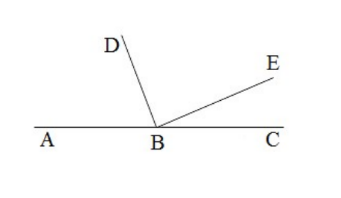
\includegraphics[align=t, width=\linewidth]{../../../../exercises/lists/pics/arofikinM9L3-1}
		\end{minipage}
		\item Сравните: \begin{tasks}(2)
			\task \( 3 \) км и \( 2 974 \) м
			\task \( 912 \) кг и \( 8 \) ц
		\end{tasks}
		\item Найдите значение выражения: \( (4,1 - 0,66 : 1,2) \cdot0,6 \).
		\item Ширина прямоугольного параллелепипеда равна \( 4 \) см, что составляет \( \dfrac{8}{15} \) его длины, а высота составляет \( 40\% \) длины. Вычислите объем параллелепипеда.
		\item Выполните действия: \( 20 : \left( \mfrac{6}{3}{14}+\mfrac{1}{11}{14}  \right) - \left( \mfrac{4}{1}{4}-\mfrac{2}{3}{4} \right):5\)
		\item Среднее арифметическое четырёх чисел равно \( 1,4 \), а среднее арифметическое трёх других
		чисел --- \( 1,75 \). Найдите среднее арифметическое этих семи чисел.
		\item Решите уравнение: \( 21,3 - y = 9,7 \).
		\item Сад прямоугольной формы имеет длину \( 40 \) м и ширину \( 30 \) м. Сливы занимают \( \dfrac{5}{12} \) сада. Какова площадь участка сада, засаженного сливами?
		\item Миша шёл из одного села в другое \( 0,7 \) ч по полю и \( 0,9 \) ч через лес, пройдя всего \( 5,31 \) км. С какой скоростью шёл Миша через лес, если по полю он двигался со скоростью \( 4,5 \) км/ч?
	\end{listofex}
\end{class}
%END_FOLD

%BEGIN_FOLD % ====>>_____ Занятие 4 _____<<====
\begin{class}[number=4]
	\begin{listofex}
		\item Занятие 4
	\end{listofex}
\end{class}
%END_FOLD

%BEGIN_FOLD % ====>>_ Домашняя работа 2 _<<====
\begin{homework}[number=2]
	\begin{listofex}
		\item Найти значение выражения \( 47,6\cdot 0,9 - 8,2\cdot 4,9 \).
		\item Вычислите: \( \mfrac{5}{6}{13}+\left( \mfrac{10}{12}{13}-2-\mfrac{2}{3}{13} \right) \)
		\item Одна сторона прямоугольника равна \( 21 \) см, а соседняя – на \(  9 \) см длиннее. Найдите периметр и площадь прямоугольника.
		\item Вычислите объём прямоугольного параллелепипеда, измерения которого равны \( 8 \) см, \( 5 \) см, \( 9 \) см.
		\item Гусеница за \( 6 \) мин проползла \( \dfrac{5}{9} \) м. С какой скоростью ползёт гусеница?
	\end{listofex}
\end{homework}
%END_FOLD

%BEGIN_FOLD % ====>>_____ Занятие 5 _____<<====
\begin{class}[number=5]
	\begin{listofex}
		\item Сравните:
		\begin{tasks}(3)
			\task \( \dfrac{6}{18} \) и \( \dfrac{5}{18} \)
			\task \( \dfrac{8}{9} \) и \( \dfrac{10}{9} \)
			\task \( \dfrac{10}{25} \) и \( \dfrac{1}{25} \)
			\task \( \dfrac{31}{41} \) и \( \dfrac{21}{41} \)
			\task \( \dfrac{9}{7} \) и \( \dfrac{7}{7} \)
			\task \( \dfrac{22}{70} \) и \( \dfrac{50}{70} \)
		\end{tasks}
		\item Сравните:
		\begin{tasks}(3)
			\task \( \dfrac{5}{17} \) и \( \dfrac{5}{21} \)
			\task \( \dfrac{12}{8} \) и \( \dfrac{12}{16} \)
			\task \( \dfrac{25}{26} \) и \( \dfrac{25}{71} \)
			\task \( \dfrac{10}{52} \) и \( \dfrac{10}{63} \)
			\task \( \dfrac{81}{100} \) и \( \dfrac{81}{99} \)
			\task \( \dfrac{2}{20} \) и \( \dfrac{2}{30} \)
		\end{tasks}
		\item Сравните: \begin{tasks}(3)
			\task \( 12,8 \) и \( 7,8 \)
			\task \( 0,08 \) и \( 0,8 \)
			\task \( 4,44 \) и \( 4,4 \)
			\task \( 12,760 \) и \( 12,76 \)
			\task \( 43,09 \) и \( 43,4 \)
			\task \( 76,098 \) и \( 76,095 \)
		\end{tasks}
		\item Представьте число в виде неправильной дроби: \begin{tasks}(4)
			\task \( \mfrac{4}{1}{3} \)
			\task \( \mfrac{5}{2}{6} \)
			\task \( \mfrac{12}{3}{5} \)
			\task \( \mfrac{3}{6}{7} \)
			\task \( \mfrac{10}{10}{11} \)
			\task \( \mfrac{5}{16}{20} \)
			\task \( \mfrac{14}{4}{5} \)
			\task \( \mfrac{25}{1}{2} \)
		\end{tasks}
		\item Выделите целую часть. Запишите ответ в виде смешанного числа.
		\begin{tasks}(3)
			\task \( \dfrac{98}{7} \)
			\task \( \dfrac{132}{12} \)
			\task \( \dfrac{505}{57} \)
			\task \( \dfrac{234}{45} \)
			\task \( \dfrac{98}{10} \)
			\task \( \dfrac{145}{9} \)
		\end{tasks}
		\item Вычислите: \quad \( \left( \mfrac{3}{1}{2}:\mfrac{2}{2}{3}+\mfrac{4}{2}{4}:\mfrac{2}{2}{3} \right)\cdot\mfrac{4}{4}{5} \)
		\item Вычислите: \\\ \( 0,5\cdot\mfrac{9}{1}{2}-\left(  \left( 2,25+\dfrac{3}{4}-2,5-\dfrac{1}{2} \right)\cdot\mfrac{5}{5}{9}+\dfrac{3}{4} \right)-\mfrac{3}{3}{4}+\mfrac{7}{1}{8}:\dfrac{1}{2} \)
		\item В первый день турист прошел 
		\( \dfrac{2}{5} \)
		намеченного пути, а во второй – оставшиеся \( 15 \) км. 
		Каков путь туриста?
	\end{listofex}
\end{class}
%END_FOLD

%BEGIN_FOLD % ====>>_____ Занятие 6 _____<<====
\begin{class}[number=6]
	\begin{listofex}
		\item Вычислите \begin{tasks}(1)
			\task \( 1,2:4+2,3\cdot(3,72-2,42)-1,44:1,2 \) 
			\task \( (6,9+7,9\cdot(4,3-2,1))\cdot1,5-30,72 \) 
		\end{tasks}  
		\item Длина куба равна \( 14,1 \). Найдите его объём.
		\item Все стороны семиугольника имеют длину \( 9,47 \) см. Найдите периметр фигуры.
		\item Ширина прямоугольного параллелепипеда, равная \( 54 \) см, на \( 16 \) см больше его высоты и в \( 6 \) раз больше его длины. Найдите объём параллелепипеда.
		\item Ширина прямоугольника \( 5,15 \) см, а длина в \( 2 \) раза больше. Найдите площадь и периметр данного прямоугольника?
		\item Площадь прямоугольника \( 42 \) см\( ^{2} \), ширина его равна \( 6 \) см. Чему равна длина прямоугольника?
		\item Ширина прямоугольника равна \( 5,2 \) см, а его длина на \( 2,15 \) см больше ширины. Периметр прямоугольника на \( 9,7 \) см больше периметра квадрата. Найдите сторону квадрата.
		\item Длина первого отрезка \( 12,9 \) см. Он в \( 3 \) раза длиннее, чем второй, а третий на \( 6,24 \) см короче, чем первый и второй вместе. Найдите длину каждого отрезка.
		\item Аквариум имеет размеры \( 60\times20\times50 \) см. Сколько литров воды нужно влить в аквариум, чтобы уровень воды был ниже верхнего края аквариума на \( 10 \) см? (\( 1 \) л =\( 1000 \) см\( ^3 \))
		\item Если сторону квадрата, периметр которого \( 36,9 \) см, уменьшить в 3 раза, то получится ширина прямоугольника, периметр которого \( 42,8 \) см. Найдите длину этого прямоугольника и вычислите его площадь.
	\end{listofex}
\end{class}
%END_FOLD

%BEGIN_FOLD % ====>>_ Домашняя работа 3 _<<====
\begin{homework}[number=3]
	\begin{listofex}
		\item Вычислите:
		\begin{tasks}(2)
			\task \( \mfrac{23}{3}{7}+\dfrac{2}{7} \)
			\task \( \dfrac{7}{10} - \dfrac{2}{5}\cdot\dfrac{1}{2}\)
			\task \( \mfrac{4}{2}{9}-\mfrac{2}{6}{9} \)
			\task \( \dfrac{2}{3}\cdot\dfrac{1}{3}+\dfrac{1}{9} \)
			\task \( \mfrac{4}{7}{9}\cdot\mfrac{1}{2}{3}-\dfrac{3}{27} \)
			\task \( \dfrac{42}{45}-\dfrac{33}{45} \)
			\task \( \mfrac{1}{1}{11}\cdot2+3\)
			\task \( 4+\dfrac{3}{8}-\mfrac{2}{2}{8} \)
		\end{tasks}
		\item Длина дороги \( 84 \) км. За первый день бригада рабочих отремонтировала \(\dfrac{ 3}{14} \) дороги, а за второй день --- \( \dfrac{5}{14} \) дороги. Сколько километров осталось отремонтировать? 
	\end{listofex}
\end{homework}
%END_FOLD

%BEGIN_FOLD % ====>>_____ Занятие 7 _____<<====
\begin{class}[number=7]
	\begin{listofex}
		\item Вычислить:
		\begin{tasks}
			\task \( 4,735\cdot0,5+14,95\cdot1,3+2,121\cdot0,7 \)
			\task \( (0,578+2,172)\cdot(1,823+0,117)-1,711\cdot(0,418+1,382) \)
			\task \( 3,006-0,0417\cdot3-0,875\cdot0,4 \)
		\end{tasks}
		\item Вычислить:
		\begin{tasks}(4)
			\task \( 1,8\cdot5,5 \)
			\task \( 41,7\cdot6,05 \)
			\task \( 8,42\cdot9,9 \)
			\task \( 6,703\cdot2,45 \)
			\task \( 55,3\cdot3,81 \)
			\task \( 6,321\cdot7,8 \)
			\task \( 32,4\cdot103,5 \)
			\task \( 8,05\cdot8,05 \)
		\end{tasks}
		\item Вычислите:
		\begin{tasks}(4)
			\task \( 0,5\cdot10 \)
			\task \( 0,15\cdot10000 \)
			\task \( 50,265\cdot10 \)
			\task \( 21,598\cdot1000 \)
			\task \( 9,56\cdot50 \)
			\task \( 8,532\cdot1200 \)
			\task \( 9,123\cdot15000 \)
			\task \( 24,1\cdot130000 \)
		\end{tasks}

	\end{listofex}
\end{class}
%END_FOLD

%BEGIN_FOLD % ====>>_ Проверочная работа _<<====
\begin{class}[number=8]
	\begin{listofex}
		\item Вычислите: 
		\begin{tasks}(1)
			\task \( \left( 13-\mfrac{8}{5}{12} \right)+\left( \mfrac{17}{1}{12}-\mfrac{16}{4}{12} \right) \)
			\task \( \left( \mfrac{63}{2}{9}+\mfrac{3}{8}{9} \right)-\left( 13-\mfrac{10}{5}{9} \right) \)
			\task \( \mfrac{2}{1}{3}\cdot\mfrac{4}{1}{3}-\mfrac{8}{4}{3}:3 \)
			\task \( \left( \dfrac{5}{4}\cdot\mfrac{2}{1}{6}\cdot\dfrac{5}{2}-1 \right):1-\dfrac{1}{2}\cdot\mfrac{1}{3}{8}\cdot\dfrac{2}{3} \)
		\end{tasks}
		\item Выполните действия:
		\begin{tasks}(1)
			\task \( 11,47+(3,89-2,11)-4,416+3,711 \)
			\task \( 3,16+(7,84-4,181)-3,11+14,816 \)
			\task \( 1,49+(6,13-4,12)-0,5+7,289 \)
		\end{tasks}
		\item Вычислите:
		\begin{tasks}(3)
			\task \( 23,4\cdot100 \)
			\task\( 4,5 \cdot100 \)
			\task \( 2,345\cdot100 \)
			\task\( 8,09\cdot0,001 \) 
			\task\( 25,043 \cdot0,001  \)
			\task\( 29,01\cdot0,001   \)
		\end{tasks}
		
		
	\end{listofex}
\end{class}
%END_FOLD

%BEGIN_FOLD % ====>>_ Домашняя работа 4 _<<====
\begin{homework}[number=4]
	\begin{listofex}
		\item Вычислите:
		\begin{tasks}(2)
			\task \( 0,763-0,321+5,8 \)
			\task \( 10,5-6,957+11,87 \)
		\end{tasks}
		\item Вычислите 
		\begin{tasks}(4)
			\task \( 1,6\cdot10 \)
			\task \( 5,8\cdot100 \)
			\task \( 15,3\cdot200 \)
			\task \( 87,701\cdot 140 \)
		\end{tasks}
		\item Вычислите 
		\begin{tasks}(3)
			\task \( 440,8\cdot0,001 \)
			\task \( 79,22\cdot31,59 \)
			\task \( 84,102\cdot13,4 \)
		\end{tasks}
		\item Бассейн имеет форму прямоугольника со сторонами \( 5,32 \) м и \( 4,74 \) м. Чему равна его площадь?
		\item Все стороны семиугольника имеют длину \( 9,47 \) см. Найдите периметр фигуры.
	\end{listofex}
\end{homework}
%END_FOLD